\documentclass{article}
\linespread{1.3}
\usepackage[margin=50pt, headheight=100pt, headsep=5pt]{geometry}
\usepackage{amsmath, amssymb, amsthm, tikz, fancyhdr, float, graphicx, spverbatim, systeme}
\pagestyle{fancy}
\renewcommand{\headrulewidth}{0pt}
\newcommand{\changefont}{\fontsize{15}{15}\selectfont}

\fancypagestyle{firstpageheader}{
  \fancyhead[R]{
    \changefont
    \parbox[t]{4cm}{ % Adjust width as needed
      Michael Huang\\
      EN.625.740.81\\
      Homework 6
    }
  }
}

\begin{document}

\thispagestyle{firstpageheader}
{\Large 

\section*{1.}

\subsection*{(a)} 
Show that the distance from the hyperplane \(g(\mathbf{x}) = \mathbf{w}^\mathbf{T} \mathbf{x} + w_0 = 0\) to the point \(\mathbf{x}_a\) is \(|g(\mathbf{x}_a)| / \lVert \mathbf{w} \rVert\) by minimizing \(\lVert \mathbf{x} - \mathbf{x}_a \rVert^2\) subject to the constraint \(g(\mathbf{x}) = 0\). \\ \\
We aim to show the statement by minimizing \(\lVert \mathbf{x} - \mathbf{x}_a \rVert^2\) with \(g(\mathbf{x}) = 0\). We build the corresponding Lagrangian which we can then attempt to minimize:
\[
  L(\mathbf{x}, \lambda) = f(\mathbf{x}) + \lambda g(\mathbf{x})
\]
\[
  = \lVert \mathbf{x} - \mathbf{x}_a \rVert^2 + \lambda \cdot (\mathbf{w}^\mathbf{T} \mathbf{x} + w_0)
\]
We can cheat a bit and multiple the first term by \(\frac{1}{2}\) to make taking the derivative and then solving easier; this is fine since we are solving for \(\mathbf{x}\) rather than the value of the minimum itself, so we don't need to account for this later. 
\[
  = \frac{1}{2} \cdot \lVert \mathbf{x} - \mathbf{x}_a \rVert^2 + \lambda \cdot (\mathbf{w}^\mathbf{T} \mathbf{x} + w_0)
\]
Let's now take the derivative with respect to \(\mathbf{x}\):
\[
  \frac{\partial}{\partial \mathbf{x}} L(\mathbf{x}) = (\mathbf{x} - \mathbf{x}_a) + \lambda \mathbf{w}
\]
and now setting to 0 to solve for the minimum:
\[
  0 = \mathbf{x} - \mathbf{x}_a + \lambda \mathbf{w}
\]
\[
  \mathbf{x} = \mathbf{x}_a - \lambda \mathbf{w}
\]
Plugging this back into the original hyperplane equation:
\[
  g(\mathbf{x}) = \mathbf{w^T x} + w_0 = 0
\]
\[
  \mathbf{w^T} (\mathbf{x}_a - \lambda \mathbf{w}) + w_0 = 0
\]
\[
  \mathbf{w^T} \mathbf{x}_a - \lambda \mathbf{w^T} \mathbf{w} + w_0 = 0
\]
\[
  (\mathbf{w^T} \mathbf{x}_a + w_0) - \lambda \lVert \mathbf{w} \rVert^2 = 0
\]
\[
  g(\mathbf{x}_a) - \lambda \lVert \mathbf{w} \rVert^2 = 0
\]
\[
  \lambda \lVert \mathbf{w} \rVert^2 = g(\mathbf{x}_a)
\]
\[
  \lambda = \frac{g(\mathbf{x}_a)}{\lVert \mathbf{w} \rVert^2}
\]
Looking back at our initial solution to the derivative of the Langrangian, from \(\mathbf{x} = \mathbf{x}_a - \lambda \mathbf{w}\), we can see that \(\mathbf{x} - \mathbf{x}_a = -\lambda \mathbf{w}\). So to find this distance, we just take the norm of this, i.e. \(\lVert -\lambda \mathbf{w} \rVert\):
\[
  \lVert -\lambda \mathbf{w} \rVert = \lVert \lambda \rVert \lVert \mathbf{w} \rVert
\]
\[
  = \frac{\lVert g(\mathbf{x}_a) \rVert}{\lVert \mathbf{w} \rVert^2}  \cdot \lVert \mathbf{w} \rVert
\]
\[
  = \frac{\lVert g(\mathbf{x}_a) \rVert}{\lVert \mathbf{w} \rVert} = \frac{g(\mathbf{x}_a)}{\lVert \mathbf{w} \rVert} 
\]
exactly as we sought to show. 

\subsection*{(b)}
Show that the projection of \(\mathbf{x}_a\) onto the hyperplane is given by 
\[
  \mathbf{x}_\mathbf{p} = \mathbf{x}_a - \frac{g(\mathbf{x}_a)}{\lVert \mathbf{w} \rVert^2} \mathbf{w}
\] \\
We kind of already showed this previously, with the last part of part (a) already using the equation 
\[
  \mathbf{x} = \mathbf{x}_a - \lambda \mathbf{w}
\]
and now taking the exact point on the hyperplane, we get 
\[
  \mathbf{x}_p = \mathbf{x}_a - \lambda \mathbf{w}
\]
and plugging in the value for \(\lambda\) which we found previously:
\[
  \mathbf{x}_p = \mathbf{x}_a - \frac{g(\mathbf{x}_a)}{\lVert \mathbf{w} \rVert^2} \mathbf{w}
\]
which is exactly what we sought to show. 

}
{\Large 

\section*{2.}
Let \(\mathbf{x_1}, \dots, \mathbf{x_n}\) be \(n\) \(q\)-dimensional samples and \(Q\) be any nonsingular positive definite \(q \times q\) matrix. Show that the vector \(\mathbf{x}\) that minimizes 
\[
  \sum_{k=1}^{n} (\mathbf{x_k} - \mathbf{x})^T Q^{-1} (\mathbf{x_k} - \mathbf{x})
\]
is the sample mean, \(\bar{\mathbf{x}} = \frac{1}{n} \sum_{k=1}^{n} \mathbf{x_k}\). \\ \\
We have the criterion function \(J(a)\) as the exact equation we are minimizing, that is, \(J(\mathbf{x}) = \sum_{k=1}^{n} (\mathbf{x_k} - \mathbf{x})^T Q^{-1} (\mathbf{x_k} - \mathbf{x})\). We therefore simply take the gradient and try to optimize accordingly:
\[
  \nabla_\mathbf{x} J(\mathbf{x}) = \sum_{k=1}^{n} 2 Q^{-1} (\mathbf{x_k} - \mathbf{x}) \cdot (0 - 1)
\]
taking the standard gradient and applying the chain rule. Continuing:
\[
  = \sum_{k=1}^{n} - 2 Q^{-1} (\mathbf{x_k} - \mathbf{x})
\]
\[
  = - 2 Q^{-1}  \sum_{k=1}^{n} (\mathbf{x_k} - \mathbf{x})
\]
And optimizing by trying to solve for the minimum by setting to 0:
\[
  - 2 Q^{-1}  \sum_{k=1}^{n} (\mathbf{x_k} - \mathbf{x}) = 0
\]
\[
  \sum_{k=1}^{n} (\mathbf{x_k} - \mathbf{x}) = 0
\]
\[
  \sum_{k=1}^{n} \mathbf{x_k} - \sum_{k=1}^{n} \mathbf{x} = 0
\]
\[
  \sum_{k=1}^{n} \mathbf{x_k} - n \mathbf{x} = 0
\]
\[
  n \mathbf{x} = \sum_{k=1}^{n} \mathbf{x_k}
\]
\[
  \mathbf{x} = \frac{1}{n} \sum_{k=1}^{n} \mathbf{x_k}
\]
which is indeed equivalent to the sample mean, as we sought to show. 

}
{\Large 

\section*{3.}
Consider a linear classifier with discriminant functions \(g_i(\mathbf{x}) = \mathbf{w}_\mathbf{i}^{\mathbf{T}} \mathbf{x} + w_{i0}, i = 1, \dots, c\). Show that the decision regions are convex by showing that if \(\mathbf{x}_1 \in \mathcal{R}_i\) and \(\mathbf{x}_2 \in \mathcal{R}_i\) then \(\lambda \mathbf{x}_1 + (1 - \lambda) \mathbf{x}_2 \in \mathcal{R}_i\) if \(0 \leq \lambda \leq 1\). \\ \\
By definition, we know that the linear machine will assign \(\mathbf{x}\) to class \(i\) if \(g_i(\mathbf{x}) > g_j(\mathbf{x})\) for all \(j \neq i\); as a byproduct of this, we also know that \(g_i(\mathbf{x_1}) > g_j(\mathbf{x_1})\) and \(g_i(\mathbf{x_2}) > g_j(\mathbf{x_2})\). As suggested by the problem statement, we aim to show that the decision regions are convex by showing that arbitrary point \(\lambda \mathbf{x_1} + (1 - \lambda) \mathbf{x_2}\) lies within the classification region with \(0 \leq \lambda \leq 1\). We substitute this value for \(\mathbf{x}\) into the linear classifier discriminant function:
\[
  g_i(\mathbf{x}) = \mathbf{w_i^T}(\lambda \mathbf{x_1} + (1 - \lambda) \mathbf{x_2}) + w_{i0} 
\]
Looking at this -- intuitively, we can see that this essentially is a complementary weighting of the two vectors since they sum to 1. We can therefore redistribute accordingly, with the bias distributed between the \(\lambda\) and \(1 - \lambda\) weights, since this still adds up to \(1 \cdot w_{i0}\):
\[
  = \lambda(\mathbf{w_i^T x_1} + w_{i0}) + (1 - \lambda)(\mathbf{w_i^T x_2} + w_{i0})
\]
and then substituting in the linear discriminant function definition accordingly:
\[
  g_i(\mathbf{x}) = \lambda g_i(\mathbf{x_1}) + (1 - \lambda) g_i(\mathbf{x_2})
\]
Based on the inequalities we previously established, we also know that \(\lambda g_i(\mathbf{x_1}) \geq \lambda g_j(\mathbf{x_1}) \), and \((1 - \lambda) g_i(\mathbf{x_2}) \geq (1 - \lambda) g_i(\mathbf{x_2})\), since multiplying by the \(0 \leq \lambda \leq 1\) doesn't change the sign of the inequality but introduces the potential of possible equality in the case that either \(\lambda\) or \(1 - \lambda\) is 0. Combining this with the actual discriminant function that we found for \(\mathbf{x}\), we see that we have 
\[
  \lambda g_i(\mathbf{x_1}) + (1 - \lambda) g_i(\mathbf{x_2}) > \lambda g_j(\mathbf{x_1}) + (1 - \lambda) g_j(\mathbf{x_2})
\]
with this being a strict inequality since only one of the weights being able to be 0, which is the only case of equality, thus leaving the other term to be a strict inequality. We already solved for this previously, so we are essentially just left with 
\[
  g_i(\mathbf{x}) > g_j(\mathbf{x})
\]
which shows us that this intermediate point satisfies the linear machine assignment rule that we first started with, which therefore indicates that indeed \(\mathbf{x} \in \mathcal{R}_i\) as we hoped to show.

}
{\Large 

\section*{4.}
In the gradient descent algorithm \(\mathbf{a}_{k+1}\) is obtained from \(\mathbf{a}_k\) by 
\[
  \mathbf{a}_{k+1} = \mathbf{a}_k - \rho_k \nabla J(\mathbf{a}_k),
\]
where \(\rho_k\) is a positive scale factor that sets the step size. Consider the criterion function
\[
  J_q(\mathbf{a}) = \sum_{\mathbf{y} \in \mathcal{Y}} (\mathbf{a}^T \mathbf{y} - b)^2
\]
where \(\mathcal{Y}(\mathbf{a})\) is the set of samples for which \(\mathbf{a}^T \mathbf{y} \leq b \). Suppose that \(\mathbf{y}_1\) is the only sample in \(\mathcal{Y}(\mathbf{a}_k)\). Show that \(\nabla J_q(\mathbf{a}_k) = 2(\mathbf{a}_k^T \mathbf{y}_1 - b)\mathbf{y}_1\) and that the matrix of second partial derivatives is given by \(D = 2\mathbf{y}_1 \mathbf{y}_1^T\). Use this to show that when the optimal \(\rho_k\) is used in the gradient descent algorithm, 
\[
  \mathbf{a}_{k+1} = \mathbf{a}_k + \frac{b - \mathbf{a}^T \mathbf{y}_1}{\|\mathbf{y}_1\|^2} \mathbf{y}_1.
\] \\
Let's first calculate the gradient as the first thing that we want to show. Because we assume that \(\mathbf{y}_1\) is the only sample, we have 
\[
  J_q (\mathbf{a}_k) = (\mathbf{a}^T \mathbf{y}_1 - b)^2
\]
and then taking the corresponding gradient:
\[
  \nabla J_q (\mathbf{a}_k) = 2(\mathbf{a}_k^T \mathbf{y}_1 - b) \cdot (\mathbf{y}_1 - 0)
\]
\[
  = 2(\mathbf{a}_k^T \mathbf{y}_1 - b)\mathbf{y}_1
\]
which matches what we expect. \\ \\
Now, we take the second derivative to check the "matrix of second partial derivatives", first isolating \(\mathbf{a}_k\) accordingly to try and get the correct form of the matrix:
\[
  \nabla J_q (\mathbf{a}_k) = 2(\mathbf{a}_k^T \mathbf{y}_1 - b)\mathbf{y}_1
\]
\[
  = (2\mathbf{a}_k^T \mathbf{y}_1 - 2b)\mathbf{y}_1
\]
\[
  = 2 \mathbf{y}_1 \mathbf{y}_1^T  \mathbf{a}_k  - 2b\mathbf{y}_1
\]
and now taking the derivative again:
\[
  D = \frac{\partial}{\partial \mathbf{a}_k} \nabla J_q (\mathbf{a}_k) = 2 \mathbf{y}_1 \mathbf{y}_1^T - 0
\]
\[
  = 2 \mathbf{y}_1 \mathbf{y}_1^T
\]
which also matches what we aimed to show as the value for \(D\). \\ \\
We now move to deriving the update rule \(\mathbf{a}_{k+1}\), first starting with finding the optimal step size \(\rho_k\). By definition in the text, we have 
\[
  \rho_k = \frac{\lVert \nabla J_q \rVert^2}{\nabla J_q^T H\nabla J_q}
\]
for which \(H\) is the Hessian, which in this case is the second partial derivative matrix \(D\). Continuing onwards:
\[
  = \frac{(2(\mathbf{a}_k^T \mathbf{y}_1 - b)\mathbf{y}_1)^T (2(\mathbf{a}_k^T \mathbf{y}_1 - b)\mathbf{y}_1)}{(2(\mathbf{a}_k^T \mathbf{y}_1 - b)\mathbf{y}_1)^T (2\mathbf{y}_1 \mathbf{y}_1^T) (2(\mathbf{a}_k^T \mathbf{y}_1 - b)\mathbf{y}_1) }
\]
\[
  = \frac{4(\mathbf{a}_k^T \mathbf{y}_1 - b)^2 \mathbf{y}_1^T \mathbf{y}_1}{8(\mathbf{a}_k^T \mathbf{y}_1 - b)^2 \mathbf{y}_1^T \mathbf{y}_1 \mathbf{y}_1^T \mathbf{y}_1}
\] 
\[
  = \frac{4(\mathbf{a}_k^T \mathbf{y}_1 - b)^2 \lVert \mathbf{y}_1 \rVert^2}{8(\mathbf{a}_k^T \mathbf{y}_1 - b)^2 \lVert \mathbf{y}_1 \rVert^4}
\] 
\[
  \rho_k = \frac{1}{2 \lVert \mathbf{y}_1 \rVert^2}
\]
And finally plugging this back in:
\[
  \mathbf{a}_{k+1} = \mathbf{a}_k - \rho_k \nabla J(\mathbf{a}_k)
\]
\[
  = \mathbf{a}_k - (\frac{1}{2 \lVert \mathbf{y}_1 \rVert^2}) \cdot 2(\mathbf{a}_k^T \mathbf{y}_1 - b) \mathbf{y}_1
\]
\[
  = \mathbf{a}_k - \frac{(\mathbf{a}_k^T \mathbf{y}_1 - b) \mathbf{y}_1}{ \lVert \mathbf{y}_1 \rVert^2}
\]
\[
  \mathbf{a}_{k+1} = \mathbf{a}_k + \frac{b - \mathbf{a}_k^T \mathbf{y}_1}{\lvert \mathbf{y} \rVert^2} \mathbf{y}_1
\]
which is exactly what we sought to show.

}
{\Large 

\section*{5.}
Show that the partial derivatives of the functions \(y_i = \exp(a_i) / \sum_k \exp(a_k)\) used in multiple class logistic discrimination are given by 
\[
  \frac{\partial y_i}{\partial a_j} = y_i (\delta_{ij} - y_j)
\]
where \(\delta_{ij} = \begin{cases}
  1, & i = j, \\ 
  0, & \text{otherwise.}
\end{cases}
\) \\ \\
We have that \(y_i = \frac{\exp(a_i)}{\sum_k \exp(a_k)}\). Generally, we use the quotient rule here:
\[
  \frac{\partial y_i}{\partial a_j} = \frac{(\frac{\partial}{\partial a_j} \exp(a_i)) \cdot (\sum_k \exp(a_k)) - \exp(a_i) \cdot \frac{\partial}{\partial a_j} \sum_k \exp(a_k)}{(\sum_k \exp(a_k))^2} 
\]
Now let's start case by case for the value of \(\delta_{ij}\). For \(i \neq j\): \\
\[
  \frac{\partial y_i}{\partial a_j} = \frac{0 \cdot (\sum_k \exp(a_k)) - \exp(a_i) \cdot \frac{\partial}{\partial a_j} \sum_k \exp(a_k)}{(\sum_k \exp(a_k))^2} 
\]
\[
  = \frac{- \exp(a_i) \cdot \frac{\partial}{\partial a_j} \sum_k \exp(a_k)}{(\sum_k \exp(a_k))^2} 
\]
\[
  = \frac{- \exp(a_i) \cdot \exp(a_j)}{(\sum_k \exp(a_k))^2} 
\]
\[
  = \frac{- \exp(a_i) }{\sum_k \exp(a_k)} \cdot \frac{\exp(a_j)}{\sum_k \exp(a_k)}
\]
and substituting back based on the form of \(y_i\) that we had before:
\[
  = -y_i y_j
\]
\[
  \frac{\partial y_i}{\partial a_j} = y_i(0 - y_j)
\]
which indeed fits the equation we aimed to find with the corresponding value of \(\delta_{ij} = 0\). Now solving for when \(i = j\):
\[
  \frac{\partial y_i}{\partial a_j} = \frac{\exp(a_i) \cdot (\sum_k \exp(a_k)) - \exp(a_i) \cdot \frac{\partial}{\partial a_j} \sum_k \exp(a_k)}{(\sum_k \exp(a_k))^2} 
\]
\[
  = \frac{\exp(a_i) \cdot (\sum_k \exp(a_k)) - \exp(a_i) \cdot \exp(a_j)}{(\sum_k \exp(a_k))^2}
\]
\[
  = \frac{\exp(a_i) \cdot (\sum_k \exp(a_k))}{(\sum_k \exp(a_k))^2} - \frac{\exp(a_i) \cdot \exp(a_j)}{\sum_k \exp(a_k) \cdot \sum_k \exp(a_k)}
\]
\[
  = \frac{\exp(a_i)}{\sum_k \exp(a_k)} - \frac{\exp(a_i)}{\sum_k \exp(a_k)} \cdot \frac{\exp(a_j)}{\sum_k \exp(a_k)}
\]
and doing the same substitutions:
\[
  = y_i - y_i \cdot y_j
\]
\[
  \frac{\partial y_i}{\partial a_j} = y_i(1 - y_j)
\]
which also fits the equation we aimed to find with corresponding value \(\delta_{ij} = 1\). 
}
{\Large 

\section*{6.}
In Module 1 we introduced nine (9) datasets. The data files are posted here in Module 9. Choose three (3) of these datasets and for each of the three:

\subsection*{(a)} 

\subsubsection*{i.}
Plot the data using a different color for each class. \\ \\
I chose the datasets 3, 5, and 7. I plotted this with the decision boundaries.

\subsubsection*{ii.}
Using the known distributions, plot the Bayes decision boundaries.
\begin{figure}[h!]
  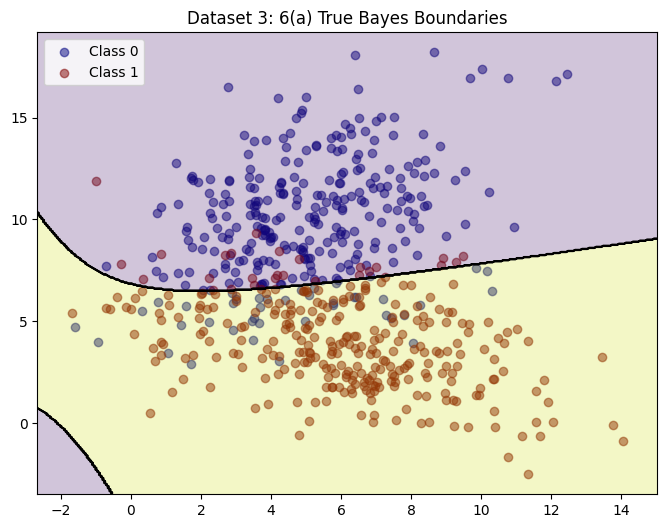
\includegraphics[width=350pt]{dataset_3_true_bayes.png}
\end{figure}
\begin{figure}[h!]
  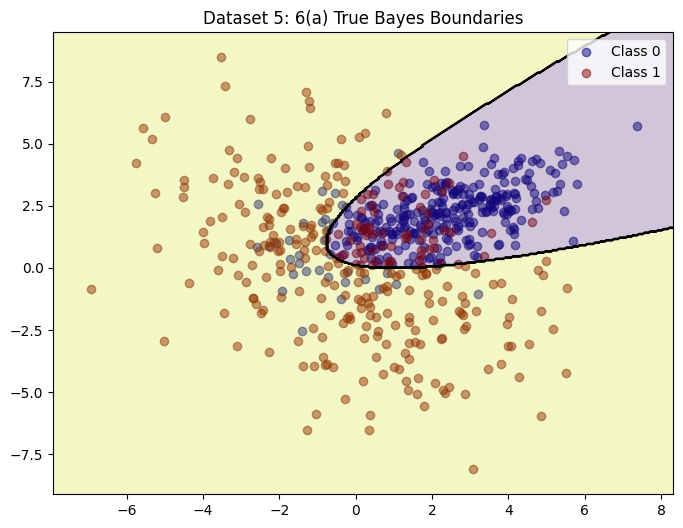
\includegraphics[width=350pt]{dataset_5_true_bayes.png}
\end{figure}
\begin{figure}[h!]
  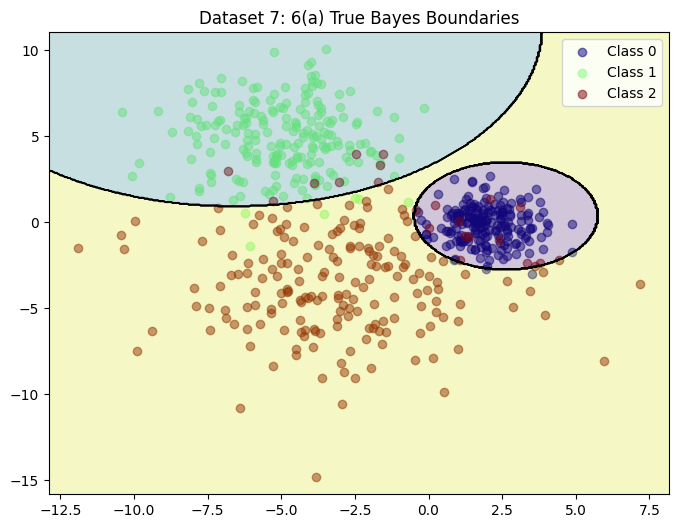
\includegraphics[width=350pt]{dataset_7_true_bayes.png}
\end{figure}

\subsection*{(b)} 
Split each dataset into 50\% training data and 50\% testing data.

\subsubsection*{i.}
Plot the testing data using a different color for each class. \\ \\
I've done all this plotting in part iv. B.

\subsubsection*{ii.}
Compute estimates for the parameters (mean and covariance) of each class.
From the outputs of the script:
\begin{spverbatim}
Dataset 3 Results
Class 0 Mean: [5.20535567 9.93734887]
Class 0 Covariance: [[5.08564406 1.24999367]
 [1.24999367 9.09153093]]
Class 1 Mean: [6.232236  3.9218732]
Class 1 Covariance: [[ 7.55745867 -2.79572445]
 [-2.79572445  4.83133451]]
Dataset 5 Results
Class 0 Mean: [2.15299033 2.05676667]
Class 0 Covariance: [[3.53022419 1.46749031]
 [1.46749031 1.63057119]]
Class 1 Mean: [0.2081042 0.1523382]
Class 1 Covariance: [[ 6.13660788 -2.27578292]
 [-2.27578292  7.24717296]]
Dataset 7 Results
Class 0 Mean: [ 1.817013  -0.1641103]
Class 0 Covariance: [[0.88612609 0.09831331]
 [0.09831331 1.10896349]]
Class 1 Mean: [-4.8462365  4.5912606]
Class 1 Covariance: [[3.06910898 0.56157984]
 [0.56157984 4.08552725]]
Class 2 Mean: [-3.0929736 -3.3100242]
Class 2 Covariance: [[ 9.45309924 -0.32012276]
 [-0.32012276  7.9429217 ]]
\end{spverbatim}

\subsubsection*{iii.}
Plot the decision boundary. \\ \\
(As previously stated, all plotting is in part iv. B.)

\subsubsection*{iv.}
Use this classifier to classify the testing data. \\ \\
(As previously stated, all plotting is in part iv. B.)

\paragraph*{A.}
Plot the decision boundary and the testing data. \\ \\
(As previously stated, all plotting is in part iv. B.)

\paragraph*{B.}
Label misclassified points.
\begin{figure}[h!]
  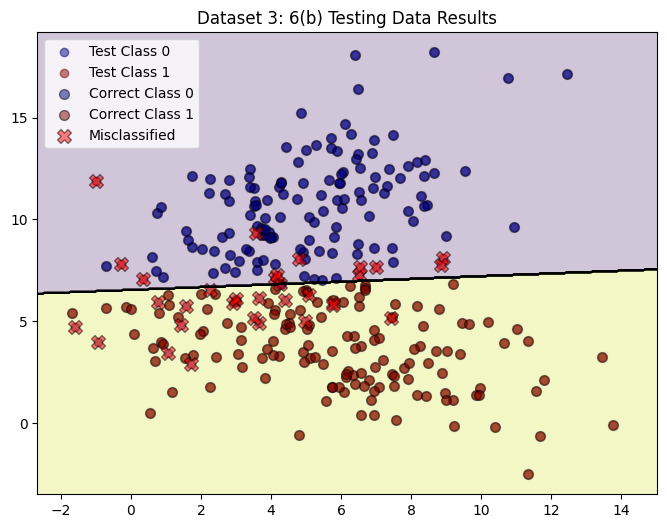
\includegraphics[width=350pt]{dataset_3_testing_data.png}
\end{figure}
\begin{figure}[h!]
  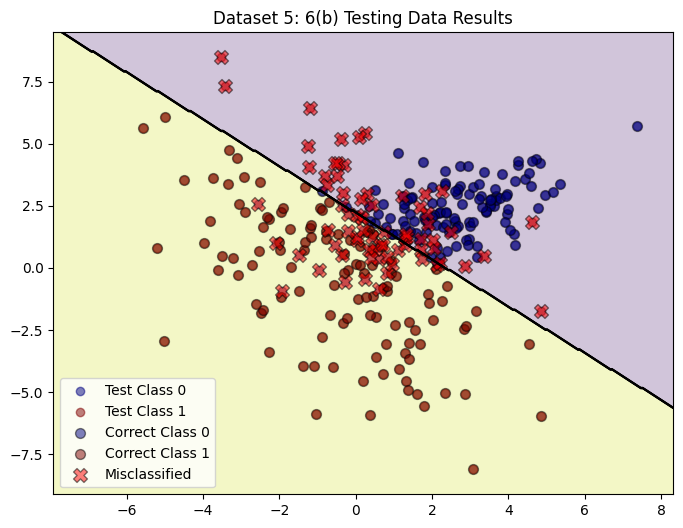
\includegraphics[width=350pt]{dataset_5_testing_data.png}
\end{figure}
\begin{figure}[h!]
  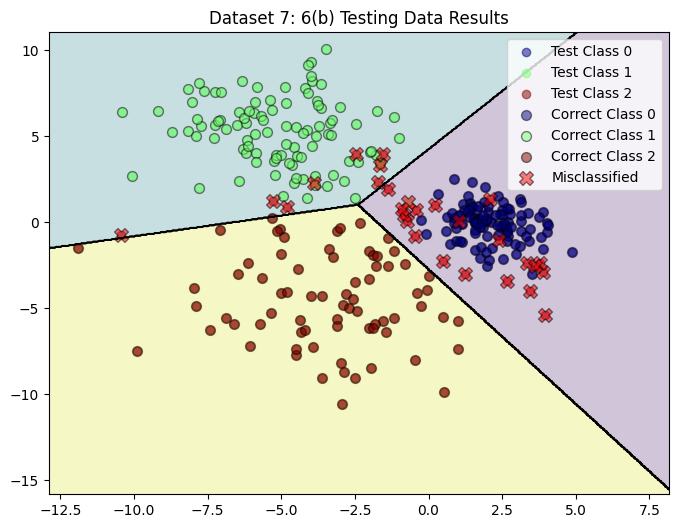
\includegraphics[width=350pt]{dataset_7_testing_data.png}
\end{figure}

\paragraph*{C.}
How well did the classifier do? Compute the percentage correct. \\ \\
From the outputs of the script:
\begin{spverbatim}
Dataset 3 Results
Percentage misclassified: 10.666666666666668%
Dataset 5 Results
Percentage misclassified: 24.0%
Dataset 7 Results
Percentage misclassified: 9.333333333333334%
\end{spverbatim}
For datasets 3, and 7, the misclassification percentage seems pretty good; however, this is much higher for Dataset 5, which had a much harder shape to do linear discrimination for. \\ \\ \\
This was the code I ran to create the above plots and find the corresponding figures:
\begin{spverbatim}
import numpy as np
import pandas as pd
import matplotlib.pyplot as plt
from scipy.stats import multivariate_normal
from sklearn.model_selection import train_test_split
from sklearn.discriminant_analysis import LinearDiscriminantAnalysis

FILE_DATASET_NAME_MAP = {
  "supervised_learning_data_3.txt" : "Dataset 3",
  "supervised_learning_data_5.txt" : "Dataset 5",
  "supervised_learning_data_7.txt" : "Dataset 7",
}

FILE_MEAN_MAP = {
  "supervised_learning_data_3.txt" : [
    np.array([5, 10]),
    np.array([6, 4]),
  ],
  "supervised_learning_data_5.txt" : [
    np.array([2, 2]),
    np.array([0, 0]),
  ],
  "supervised_learning_data_7.txt" : [
    np.array([2, 0]),
    np.array([-5, 5]),
    np.array([-3, -3]),
  ],
}

P1 = np.array([
  [np.cos(np.pi/6), np.sin(np.pi/6)], 
  [-np.sin(np.pi/6), np.cos(np.pi/6)],
])
P2 = np.array([
  [np.cos(2*np.pi/3), np.sin(2*np.pi/3)], 
  [-np.sin(2*np.pi/3), np.cos(2*np.pi/3)],
])
Q = np.array([[4, 0], [0, 9]])
P = np.array([
  [np.cos(5*np.pi/6), np.sin(5*np.pi/6)], 
  [-np.sin(5*np.pi/6), np.cos(5*np.pi/6)],
])

FILE_COVARIANCE_MAP = {
  "supervised_learning_data_3.txt" : [
    P1 @ Q @ P1.T,
    P2 @ Q @ P2.T,
  ],
  "supervised_learning_data_5.txt" : [
    P @ np.array([[4, 0], [0, 1]]) @ P.T,
    P @ np.array([[4, 0], [0, 9]]) @ P.T,
  ],
  "supervised_learning_data_7.txt" : [
    np.eye(2), 
    4 * np.eye(2), 
    9 * np.eye(2),
  ]
}



def analyze_dataset(filepath):
  df = pd.read_csv(filepath, header=None)
  x = df.iloc[:, :-1].values
  y = df.iloc[:, -1].values
  classes = np.unique(y)
  print(f"{FILE_DATASET_NAME_MAP[filepath]} Results")
  
  # Generate color values along the rainbow spectrum for the number of classes
  colors = [plt.cm.jet(i / (len(classes) - 1)) for i in range(len(classes))]

  # (a) i. Plot the data using a different color for each class.
  plt.figure(figsize=(8, 6))
  for idx, class_label in enumerate(classes):
    plt.scatter(
      x[y == class_label, 0],
      x[y == class_label, 1],
      color=colors[idx], label=f"Class {int(class_label)}", alpha=0.5
    )

  # (a) ii. Using the known distributions, plot the Bayes decision boundaries.

  mean_list = FILE_MEAN_MAP[filepath]
  covariance_list = FILE_COVARIANCE_MAP[filepath]

  # Set up numpy meshgrid which is used for shaping the decision boundaries

  x_min, x_max = x[:, 0].min() - 1, x[:, 0].max() + 1
  y_min, y_max = x[:, 1].min() - 1, x[:, 1].max() + 1
  xx, yy = np.meshgrid(np.arange(x_min, x_max, 0.05), np.arange(y_min, y_max, 0.05))
  pos = np.dstack((xx, yy))

  probabilities = [multivariate_normal(mean=mu, cov=cov).pdf(pos) for mu, cov in zip(mean_list, covariance_list)]
  Z_bayes = np.argmax(probabilities, axis=0)

  plt.contourf(xx, yy, Z_bayes, alpha=0.25)
  plt.contour(xx, yy, Z_bayes, colors="black", linewidths=1)
    
  plt.title(f"{FILE_DATASET_NAME_MAP[filepath]}: 6(a) True Bayes Boundaries")
  plt.legend()
  plt.savefig(f"dataset_{FILE_DATASET_NAME_MAP[filepath][-1]}_true_bayes.png", bbox_inches="tight")
  plt.show()
  plt.close()

  # (b) Split each dataset into 50% training data and 50% testing data. 
  x_train, x_test, y_train, y_test = train_test_split(x, y, test_size=0.5, stratify=y)

  # (b) i. Plot the testing data using a different color for each class.
  plt.figure(figsize=(8, 6))
  for idx, class_label in enumerate(classes):
    plt.scatter(
      x_test[y_test == class_label, 0],
      x_test[y_test == class_label, 1],
      color=colors[idx], label=f"Test Class {int(class_label)}", alpha=0.5
    )

  # (b) ii. Compute estimates for the parameters (mean and covariance) of each class.
  for c in classes:
    x_class = x_train[y_train == c]
    print(f"Class {int(c)} Mean: {np.mean(x_class, axis=0)}")
    print(f"Class {int(c)} Covariance: {np.cov(x_class, rowvar=False)}")

  lda = LinearDiscriminantAnalysis()
  lda.fit(x_train, y_train)
  
  y_pred = lda.predict(x_test)
  misclassified = x_test[y_pred != y_test]

  Z_linear = lda.predict(np.c_[xx.ravel(), yy.ravel()]).reshape(xx.shape)

  plt.contourf(xx, yy, Z_linear, alpha=0.25)
  plt.contour(xx, yy, Z_linear, colors="black", linewidths=1)

  for idx, class_label in enumerate(classes):
    plt.scatter(
      x_test[(y_test == class_label) & (y_pred == y_test), 0],
      x_test[(y_test == class_label) & (y_pred == y_test), 1],
      color=colors[idx], marker="o", edgecolor="k", s=50, label=f"Correct Class {int(class_label)}", alpha=0.5
    )

  if len(misclassified) > 0:
    print(f"Percentage misclassified: {len(misclassified) / len(y_pred) * 100}%")
    plt.scatter(
      misclassified[:, 0],
      misclassified[:, 1],
      color="red", marker="X", s=100, edgecolor="black", label="Misclassified", linewidths=1, alpha=0.5
    )
 
  plt.title(f"{FILE_DATASET_NAME_MAP[filepath]}: 6(b) Testing Data Results")
  plt.legend()
  plt.savefig(f"dataset_{FILE_DATASET_NAME_MAP[filepath][-1]}_testing_data.png", bbox_inches="tight")
  plt.show()
  plt.close()

analyze_dataset("supervised_learning_data_3.txt")
analyze_dataset("supervised_learning_data_5.txt")
analyze_dataset("supervised_learning_data_7.txt")
\end{spverbatim}

}

\end{document}